\documentclass[12pt,a4paper]{article}
\usepackage[a4paper,left=2cm,right=2cm,top=2.3cm,bottom=2.5cm]{geometry}
\usepackage{setspace}
\usepackage{graphicx}
\usepackage{float}
\usepackage{booktabs}
\usepackage{tabularx}
\usepackage{array}
\usepackage{enumitem}
\usepackage[numbers,sort&compress]{natbib}
\usepackage[hidelinks]{hyperref}
\usepackage{xcolor}
\usepackage{colortbl}
\definecolor{tablehead}{RGB}{30, 80, 85}
\definecolor{tablerowlight}{RGB}{246, 250, 251}
\definecolor{tablehighlight}{RGB}{224, 240, 242}
\definecolor{tableborder}{RGB}{45, 110, 115}

\usepackage{tikz}
\usetikzlibrary{arrows.meta,positioning,shapes.geometric}
\usepackage{pgfplots}
\pgfplotsset{compat=1.18}
\setlength{\parindent}{1cm}
\onehalfspacing
\newcolumntype{Y}{>{\raggedright\arraybackslash}X}
\newcolumntype{L}[1]{>{\raggedright\arraybackslash}p{#1}}
\graphicspath{{figures/}}
\title{Human Activity Recognition Using Image and Skeleton-Based Methods}

\begin{document}

\begin{titlepage}
\begin{center}
\vspace*{0.5cm}
{\large\textbf{Mini Project Report}}\\[0.35cm]
{\large on}\\[0.45cm]
{\LARGE\textbf{Human Activity Recognition Using Image and Skeleton-Based Methods}}\\[0.9cm]
{\small Submitted by}\\[0.3cm]
\begin{tabular}{lc}
\textbf{Kothapally Anjan Reddy} & 23BCS071 \\
\textbf{Babhale Rohan Laxmikant} & 23BCS026 \\
\textbf{Kshitij Shende} & 23BCS075
\end{tabular}\\[0.8cm]
{\small Under the guidance of}\\[0.2cm]
{\large\textbf{Dr. Sunil C. K.}}\\
Assistant Professor
\vfill

\includegraphics[width=2.55in]{iiit_dharwad_logo.png}\\[0.35cm]
{\Large\textbf{INDIAN INSTITUTE OF INFORMATION TECHNOLOGY DHARWAD}}\\[0.2cm]
DEPARTMENT OF COMPUTER SCIENCE AND ENGINEERING\\[0.4cm]
11 November 2026
\end{center}
\end{titlepage}

\newpage
\thispagestyle{empty}
\begin{center}\emph{\huge Certificate}\end{center}
\vspace{1.5cm}
This is to certify that the project entitled \textbf{Human Activity Recognition Using Image and Skeleton-Based Methods} is a record of the Mini Project coursework completed by the students listed below during the academic year 2026--27. The work is submitted in partial fulfilment of the requirements for the degree of Bachelor of Technology in Computer Science and Engineering.
\vspace{1.2cm}
\begin{center}
\begin{tabular}{cl}
\textbf{Roll No.} & \textbf{Name} \\
\midrule
23BCS071 & Kothapally Anjan Reddy \\
23BCS026 & Babhale Rohan Laxmikant\\
23BCS075 & Kshitij Shende
\end{tabular}
\end{center}
\vfill
\begin{flushright}
Dr. Sunil C. K.\\
(Project Supervisor)
\end{flushright}

\newpage
\pagenumbering{roman}
\tableofcontents
\newpage
\listoffigures
\newpage
\listoftables
\newpage
\pagenumbering{arabic}

\section{Introduction}
Human Activity Recognition (HAR) means identifying what action a person is doing from visual information such as images or videos. Tennis stroke recognition is a fine-grained task: many strokes look similar, and the differences can be small changes in body movement during a swing. This makes it difficult to recognize a stroke from only one or a few video frames.

This project uses the public THETIS (Three-dimensional Tennis Shots) dataset. It contains 1,980 RGB videos of 12 tennis strokes performed by 55 players. Each player performed each stroke three times. The 12 classes are backhand, backhand2hands, backhand\_slice, backhand\_\allowbreak volley, forehand\_flat, forehand\_\allowbreak openstands, forehand\_slice, forehand\_\allowbreak volley, flat\_\allowbreak service, kick\_\allowbreak service, slice\_\allowbreak service, and smash~\cite{gourgari2013thetis}.

The project was completed in two parts. The first pipeline used transfer learning with an ImageNet-pretrained ResNet50 convolutional neural network (CNN) to classify still frames from the videos. It tested one midpoint frame and three frames sampled across each video. The second pipeline was added as an extension. It used a pretrained YOLO11m-pose detector to find 17 body points in each frame, then compared a model using one midpoint pose (Model A) with a model using the full sequence of 64 resampled poses (Model B).

The videos do not show a tennis ball. The missing ball and the small differences between some strokes make the three service classes especially difficult. Another study using THETIS also reported frequent confusion among serve types and related strokes~\cite{hovad2024classification}.

To make the evaluation fair, both pipelines used a subject-wise split: all videos of one player were assigned to only one of the training, validation, or test sets. This prevents the model from seeing the same player in both training and testing. On the held-out test players, Model B reached 68.0\% average accuracy across five training runs. The report also compares this result with the photo pipeline and discusses why the comparison has limits.

\clearpage
\section{Related Work}
Human action recognition in sports video analysis represents a fine-grained subfield of computer vision. Unlike coarse human activity recognition where action categories correlate with disparate environmental backgrounds (such as a swimming pool versus a running track), athletic stroke recognition takes place within visually invariant tennis court environments. The discriminating signals reside in subtle, rapid spatio-temporal transitions of the athlete's body kinematics. This section surveys prior literature across five foundational dimensions directly informing this project: the THETIS benchmark, image-based transfer learning with residual networks, modern real-time pose estimation architectures, kinematic sequence modeling with 1D temporal convolutions, and rigorous evaluation protocols for identity-leak-free action recognition.

\subsection{The THETIS Dataset and Tennis Action Recognition Benchmarks}
Gourgari and colleagues~\cite{gourgari2013thetis} introduced the Three-dimensional Tennis Shots (THETIS) benchmark to establish a dedicated public platform for fine-grained sports action recognition. THETIS consists of 1,980 RGB video clips capturing 12 distinct tennis strokes performed by 55 human subjects (31 amateurs and 24 experienced players), with each player performing three repetitions per stroke. The taxonomy spans four backhand variations (\texttt{backhand}, \texttt{backhand2hands}, \texttt{backhand\_\allowbreak slice}, \texttt{backhand\_\allowbreak volley}), four forehand variations (\texttt{forehand\_flat}, \texttt{forehand\_\allowbreak openstands}, \texttt{forehand\_\allowbreak slice}, \texttt{forehand\_\allowbreak volley}), three service actions (\texttt{flat\_\allowbreak service}, \texttt{kick\_\allowbreak service}, \texttt{slice\_\allowbreak service}), and an overhead \texttt{smash}.

The clips were captured indoors using a Microsoft Kinect v1 sensor at a resolution of approximately $640 \times 480$ pixels and a frame rate of 17--18 frames per second, with video durations ranging from 24 to 150 frames. THETIS presents unique domain challenges: the tennis ball is not tracked due to low frame rates and motion blur, the racquet angle cannot be reliably segmented with standard appearance models, and high intra-class biomechanical variability exists between amateur and experienced players. Most critically, several strokes share nearly identical preparatory phases. For instance, flat, kick, and slice services involve similar ball-toss stances, with distinguishing biomechanics confined to wrist pronation and racquet trajectory during contact. In the original benchmark, Gourgari et al.~\cite{gourgari2013thetis} applied Bag-of-Visual-Words (BoW) models on 3D silhouettes, HOG/HOF descriptors, and Support Vector Machines (SVM), reporting accuracies between 60\% and 70\% on simplified subsets while identifying severe confusion among service classes. Furthermore, early literature predominantly relied on random clip-level splitting, which permitted footage of the same athlete to appear in both training and test partitions, inflating accuracy through player identity memorization.
\clearpage
\subsection{Image-Based Action Recognition and Deep Transfer Learning}
Deep transfer learning represents the dominant paradigm for visual recognition tasks with limited training samples. Models are initialized with feature extractors pretrained on massive image corpora such as ImageNet-1k (1.28 million images across 1,000 categories)~\cite{russakovsky2015imagenet}. The Deep Residual Network (ResNet) architecture, introduced by He et al.~\cite{he2016deep}, incorporates identity shortcut connections: $y = \mathcal{F}(x, W) + x$, where $x$ and $y$ denote the input and output activation vectors of the residual building block, and $\mathcal{F}(x, W)$ represents the residual mapping. This formulation enables effective gradient propagation through 50 or more layers without signal degradation or vanishing gradients.

Adapting static image backbones like ResNet50 to video action classification involves extracting representative keyframes. A single frame sampled at the temporal midpoint of the swing captures the impact stance, whereas a multi-frame consensus formulation samples three frames across the trajectory (at 25\%, 50\%, and 75\% of total duration) to capture preparatory, execution, and follow-through phases. We employ progressive two-phase fine-tuning: Phase 1 freezes the pretrained convolutional layers and trains only a newly attached 12-class linear head using the Adam optimizer~\cite{kingma2015adam} at learning rate 0.001; Phase 2 selectively unfreezes the deepest residual block (\texttt{layer4}) at a conservative learning rate of 0.00001 with frozen batch-normalization running statistics. However, static 2D image models heavily exploit static appearance cues (court background, lighting, player attire) rather than genuine stroke dynamics, limiting their temporal modeling capabilities.

\subsection{Human Pose Estimation and the YOLO11-Pose Framework}
Human pose estimation abstracts away irrelevant background context and athlete attire, transforming raw pixel streams into explicit anatomical landmark trajectories. Early 2D pose estimators, such as OpenPose and AlphaPose, operated as multi-stage systems requiring separate person detection bounding boxes followed by computationally demanding Gaussian heatmap regressions for keypoint localization, incurring high latency.

Modern anchor-free architectures have substantially advanced real-time pose estimation. Ultralytics YOLO11m-pose~\cite{jocher2024yolo11} integrates an efficient C3k2 convolutional backbone with Spatial Pyramid Pooling Fast (SPPF) modules and decoupled prediction heads. Directly from raw $640 \times 640$ RGB frames, the model concurrently regresses bounding boxes and 17 standardized COCO keypoint coordinates~\cite{lin2014microsoft} (nose, eyes, ears, shoulders, elbows, wrists, hips, knees, ankles) along with joint visibility confidences as coordinate-confidence tuples $(x, y, c)$. Employing YOLO11m-pose on THETIS is methodologically critical: although the original dataset included raw Kinect skeletons, those joint streams were incomplete, suffered from severe depth sensor dropouts, and lacked standardized coordinate formatting. Applying YOLO11m-pose across the RGB clips recovers a continuous, reliable 2D skeletal representation directly from high-resolution video archives.
\clearpage
\subsection{Kinematic Sequence Modeling and Temporal 1D Convolutional Networks}
Representing human movement as spatio-temporal coordinate sequences isolates pure biomechanics from visual background noise. Extracted landmark sequences form a temporal tensor of shape $T \times 17 \times 2$. Because raw clips span 24 to 150 frames, uniform linear resampling standardizes each clip to $T = 64$ evenly spaced time steps. Spatial normalization centers coordinates on the hip midpoint and scales them by the video's median shoulder-to-hip torso distance. Unreliable joints (confidence below 0.5) or tracking dropouts are repaired via temporal linear interpolation.

To classify the normalized 64-step sequence, 1D Temporal Convolutional Neural Networks (1D-CNNs) offer compelling advantages over recurrent architectures (LSTM/GRU) and Graph Convolutional Networks (ST-GCN)~\cite{yan2018spatial}. While recurrent models face sequential execution bottlenecks and ST-GCNs introduce substantial structural overhead sensitive to joint noise, 1D-CNNs slide convolutional filters across time in parallel. Their hierarchical temporal receptive fields efficiently capture joint velocities, accelerations, and multi-phase stroke mechanics with low computational complexity.

\subsection{Evaluation Protocols, Subject-Wise Splitting, and Temporal Order Ablation}
A pervasive pitfall in sports action recognition is random clip-level splitting. When clips of the same player are distributed across training and test partitions, deep visual models easily memorize athlete identity, clothing, and court habits (identity leakage), inflating benchmark scores without learning genuine stroke biomechanics. True generalization requires strict subject-wise partitioning: all recordings of any given athlete are assigned exclusively to training, validation, or test sets.

Additionally, a fundamental question in kinematic modeling is whether a network genuinely captures chronological motion dynamics or merely acts as an ensemble over static postures (a ``bag-of-poses'' effect). To verify the contribution of temporal order, a randomized temporal shuffle control experiment is essential. Randomly permuting the 64 time steps during training and inference preserves identical posture statistics while stripping chronological dynamics. Comparing the ordered model against this shuffled baseline rigorously quantifies the performance gain provided by temporal progression.
\clearpage
\subsection{Comparative Synthesis and Project Novelty}
Table~\ref{tab:prior-work-comparison} summarizes prior investigations on THETIS and sports action recognition in relation to our dual-pipeline project.

\begin{table}[H]
\centering
\footnotesize
\setlength{\tabcolsep}{2.5pt}
\renewcommand{\arraystretch}{0.98}
\arrayrulecolor{tableborder}
\caption{Comparative landscape of prior research on THETIS versus our proposed framework.}
\label{tab:prior-work-comparison}
\begin{tabularx}{\textwidth}{L{2.1cm} L{1.7cm} L{1.9cm} L{1.8cm} L{1.9cm} Y}
\toprule
\rowcolor{tablehead}
\textcolor{white}{\textbf{Study}} & \textcolor{white}{\textbf{Modality}} & \textcolor{white}{\textbf{Model}} & \textcolor{white}{\textbf{Split}} & \textcolor{white}{\textbf{Strategy}} & \textcolor{white}{\textbf{Key Findings and Observations}} \\
\midrule
Gourgari et al.~\cite{gourgari2013thetis} (2013) & RGB, Depth, Kinect Joints & BoW + HOG/HOF with SVM & Random clip-level split & Static histogram aggregation & $\approx$60--70\% on subsets; high serve confusion; native Kinect skeletons incomplete. \\
\rowcolor{tablerowlight}
Hovad et al.~\cite{hovad2024classification} (2024) & RGB Video Volumes & SlowFast (Dual 3D-CNN) & Standard THETIS clips & Dual-framerate 3D convolution & $\approx$74\% top-1; high compute footprint; serve classes heavily confused; attire bias. \\
Carreira \&\ Zisserman~\cite{carreira2017quo} (2017) & RGB Video Volumes & I3D (Two-stream 3D) & Random clip splits & Spatio-temporal 3D convolution & Strong video baseline, but highly prone to athlete identity memorization on small cohorts. \\
\rowcolor{tablerowlight}
Yan et al.~\cite{yan2018spatial} (2018) & 2D Skeletons & ST-GCN (Graph CNN) & Subject split (NTU) & Graph spatial-temporal conv & Robust graph modeling; sensitive to joint jitter in fine swing trajectories. \\
\midrule
\rowcolor{tablehighlight}
\textbf{Ours (Photo Pipeline)} & RGB Still Frames & ResNet50 (ImageNet transfer) & \textbf{Strict Subject-Wise} (39/8/8) & Frame score averaging ($K=3$) & 30.56\% (1-frame), 33.33\% (3-frame avg); reveals severe limits of static appearance cues. \\
\rowcolor{tablehighlight}
\textbf{Ours (Skeleton Pipeline)} & 2D Kinematic Sequence & Model A (MLP) \& Model B (1D-CNN) & \textbf{Strict Subject-Wise} (39/8/8) & 1D-CNN ($T=64$) + Shuffle Control & \textbf{68.0\% $\pm$ 1.4\%} (Model B); eliminates identity leakage; isolates motion order (+11.1\% gain). \\
\bottomrule
\end{tabularx}
\end{table}

This project delivers four key technical novelties relative to prior literature:
\begin{enumerate}[topsep=0pt,itemsep=0pt,parsep=0pt,partopsep=0pt]
\item \textbf{RGB-to-Kinematic Pose Foundation Recovery}: Leveraging YOLO11m-pose on RGB videos, recovering clean 17-point coordinate sequences with hip-centering and median torso scaling.
\item \textbf{Strict Subject-Wise Athlete Partitioning}: Implementing an uncompromised 39/8/8 player split stratified by skill level, completely eliminating player identity and clothing leakage.
\item \textbf{Controlled Spatial vs.\ Kinematic Comparison}: Directly benchmarking ImageNet transfer learning against kinematic sequence modeling on identical held-out athletes.
\item \textbf{Rigorous Empirical Temporal Order Verification}: Executing a controlled shuffle test (56.9\% shuffled vs.\ 68.0\% ordered), proving the +11.1\% gain from chronological dynamics.
\end{enumerate}
\clearpage
\section{Data and Methods}
\subsection{Dataset and class labels}
THETIS contains 55 players: 31 beginners and 24 more experienced players. Every player performed each of 12 strokes three times, giving 1,980 RGB videos. The clips were recorded with a Kinect camera at approximately 640 by 480 pixels and 17--18 frames per second. Their lengths range from about 24 to 150 frames~\cite{gourgari2013thetis}.

\vspace{0.6em}
\begin{table}[H]
\centering
\small
\setlength{\tabcolsep}{8pt}
\renewcommand{\arraystretch}{1.25}
\arrayrulecolor{tableborder}
\caption{Tennis stroke classes used in the project.}
\label{tab:stroke-classes}
\begin{tabularx}{\textwidth}{lY lY}
\toprule
\rowcolor{tablehead}
\textcolor{white}{\textbf{Group}} & \textcolor{white}{\textbf{Classes}} & \textcolor{white}{\textbf{Group}} & \textcolor{white}{\textbf{Classes}} \\
\midrule
\rowcolor{tablerowlight}
Backhand & \texttt{backhand}, \texttt{backhand2hands}, \texttt{backhand\_\allowbreak slice}, \texttt{backhand\_\allowbreak volley} & Forehand & \texttt{forehand\_flat}, \texttt{forehand\_\allowbreak openstands}, \texttt{forehand\_slice}, \texttt{forehand\_\allowbreak volley} \\
Serve & \texttt{flat\_\allowbreak service}, \texttt{kick\_\allowbreak service}, \texttt{slice\_\allowbreak service} & Overhead & \texttt{smash} \\
\bottomrule
\end{tabularx}
\end{table}

\subsection{Subject-wise split}
The split was created once with seed 42 and reused in both pipelines. The split script separated beginner and experienced players before assigning people to groups. This gave 39 training players, 8 validation players, and 8 test players. No player appears in more than one group.

\vspace{0.6em}
\begin{table}[H]
\centering
\small
\setlength{\tabcolsep}{8pt}
\renewcommand{\arraystretch}{1.25}
\arrayrulecolor{tableborder}
\caption{Subject-wise dataset split.}
\label{tab:split}
\begin{tabular}{lrrr}
\toprule
\rowcolor{tablehead}
\textcolor{white}{\textbf{Set}} & \textcolor{white}{\textbf{Players}} & \textcolor{white}{\textbf{Videos}} & \textcolor{white}{\textbf{Videos per class}} \\
\midrule
\rowcolor{tablerowlight}
Training & 39 & 1,404 & 117 \\
Validation & 8 & 288 & 24 \\
\rowcolor{tablehighlight}
\textbf{Test (Held-Out)} & 8 & 288 & 24 \\
\bottomrule
\end{tabular}
\end{table}

\subsection{ResNet50 photo pipeline}
The photo pipeline first extracted frames from each RGB video. One version used the middle frame. A second version sampled frames at 25\%, 50\%, and 75\% of the video. The extracted images were copied into training, validation, and test folders using the shared player split.

The dataset loader resized images to 224 by 224 pixels, converted them to tensors, and applied ImageNet normalization. During training only, it used random horizontal flips, rotations up to 15 degrees, and brightness and contrast changes. The validation and test images received resizing and normalization only.

The model started with ImageNet-pretrained ResNet50 weights. The final layer was replaced with a 12-class output layer. Training had two phases. First, only the new output layer was trained while the rest of the network was frozen, using Adam with a learning rate of 0.001. Next, the last residual block and the output layer were trained at a lower learning rate of 0.00001. Batch-normalization statistics were kept fixed. Validation accuracy was used to save the best model and stop training when it stopped improving. Adam is an optimization method used to update a model's weights during training~\cite{kingma2015adam}.

For the three-frame setup, frames were first scored separately. A separate per-video result was calculated by averaging the three predicted class-probability values for each clip and choosing the highest average. This combines predictions; it does not train the model to understand frame order.

\subsection{Skeleton pipeline}
The supplied THETIS skeleton videos were incomplete and were not joint-coordinate files suitable for this model. The project therefore extracted new poses from the RGB videos using YOLO11m-pose at an image size of 640. The detector identifies 17 body points per frame, including the nose, eyes, ears, shoulders, elbows, wrists, hips, knees, and ankles~\cite{jocher2024yolo11,lin2014microsoft}.

\begin{figure}[H]
\centering
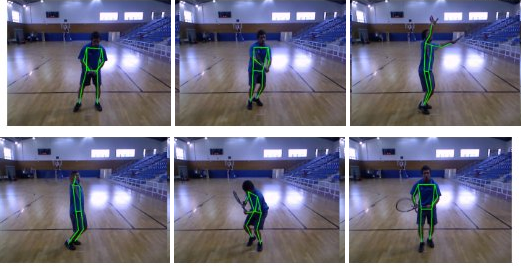
\includegraphics[width=0.88\textwidth]{image_2.png}
\caption{Example of YOLO11m-pose keypoint detection overlaid on sampled frames of a smash video (p35\_smash\_s1).}
\label{fig:pose-overlay}
\end{figure}

During extraction, the largest person box was selected in each frame. Quality checks later found videos where tracking jumped to a bystander. Selected videos were re-extracted by tracking all people and following the chosen player through the clip. A cleaning step marked frames as unreliable if the person was missing, too few key joints had confidence above 0.5, the detected body size changed sharply, or the hip midpoint jumped compared with nearby frames.

Unreliable joint positions were estimated from nearby valid times by linear interpolation. The coordinates were then centered on the midpoint between the hips and divided by the video’s median shoulder-to-hip distance. This reduces the effect of where the player stands in the frame and how large they appear. Each video was resampled to 64 evenly spaced time steps. Each time step contains a pose with 17 points and two coordinates per point.

\begin{figure}[H]
\centering
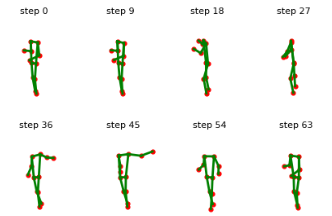
\includegraphics[width=0.68\textwidth]{image_1.png}
\caption{Example of a normalized skeleton sequence (p1\_backhand\_s1), shown at steps 0, 9, 18, 27, 36, 45, 54, and 63 of the 64 resampled time steps.}
\label{fig:pose-sequence}
\end{figure}

Model A receives only the pose at the middle of the swing. Its 17 points provide 34 coordinate values. Model B receives all 64 poses in order and uses a small 1D convolutional neural network (1D-CNN) to classify the stroke. The final models use no swing-duration input.

During training, the pose sequences could be mirrored left to right, scaled slightly, and changed with small coordinate noise. Mirroring also swaps left and right body-point labels. These changes were applied to training data only.

\subsection{Validation and test procedure}
Training videos were used to teach the models. Validation videos were used during development to compare settings and decide when to stop training. Test videos were kept aside for the final evaluation. Phase 4b compared six skeleton model settings using five seeds, 42--46. Phase 5 trained fresh models for the final comparison, again using five seeds. The reported skeleton results are the mean and standard deviation of the five test accuracies. The seeds change random training choices; they do not change the player split.

\clearpage
\section{Results and Discussions}
\subsection{Validation results}
The one-frame ResNet50 run reached a best validation accuracy of 26.39\%. The three-frame run reached 20.25\% validation accuracy at epoch 19. The curves below show how training and validation accuracy changed during both runs.

\begin{figure}[H]
\centering
\begin{minipage}{0.475\textwidth}
\centering
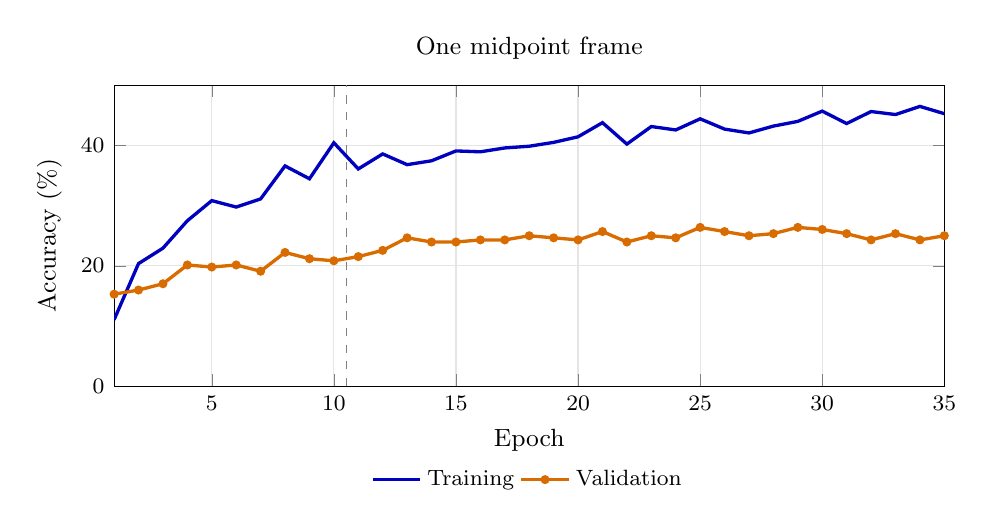
\begin{tikzpicture}
\begin{axis}[width=\textwidth,height=5.4cm,xmin=1,xmax=35,ymin=0,ymax=50,
 xlabel={Epoch},ylabel={Accuracy (\%)},title={One midpoint frame},
 grid=major,grid style={gray!20},tick label style={font=\footnotesize},
 label style={font=\small},title style={font=\small},
 legend style={font=\footnotesize,at={(0.5,-0.24)},anchor=north,legend columns=2,draw=none}]
\addplot[blue!75!black,very thick] coordinates { (1,11.040) (2,20.370) (3,22.934) (4,27.493) (5,30.840) (6,29.772) (7,31.125) (8,36.610) (9,34.473) (10,40.456) (11,36.111) (12,38.604) (13,36.823) (14,37.464) (15,39.103) (16,38.960) (17,39.601) (18,39.886) (19,40.527) (20,41.453) (21,43.803) (22,40.242) (23,43.162) (24,42.593) (25,44.444) (26,42.735) (27,42.094) (28,43.234) (29,44.017) (30,45.726) (31,43.661) (32,45.655) (33,45.157) (34,46.510) (35,45.299) };
\addlegendentry{Training}
\addplot[orange!85!black,very thick,mark=*,mark size=1pt] coordinates { (1,15.278) (2,15.972) (3,17.014) (4,20.139) (5,19.792) (6,20.139) (7,19.097) (8,22.222) (9,21.181) (10,20.833) (11,21.528) (12,22.569) (13,24.653) (14,23.958) (15,23.958) (16,24.306) (17,24.306) (18,25.000) (19,24.653) (20,24.306) (21,25.694) (22,23.958) (23,25.000) (24,24.653) (25,26.389) (26,25.694) (27,25.000) (28,25.347) (29,26.389) (30,26.042) (31,25.347) (32,24.306) (33,25.347) (34,24.306) (35,25.000) };
\addlegendentry{Validation}
\addplot[gray,dashed,forget plot] coordinates {(10.5,0)(10.5,50)};
\end{axis}
\end{tikzpicture}
\end{minipage}%\hfill%
\begin{minipage}{0.475\textwidth}
\centering
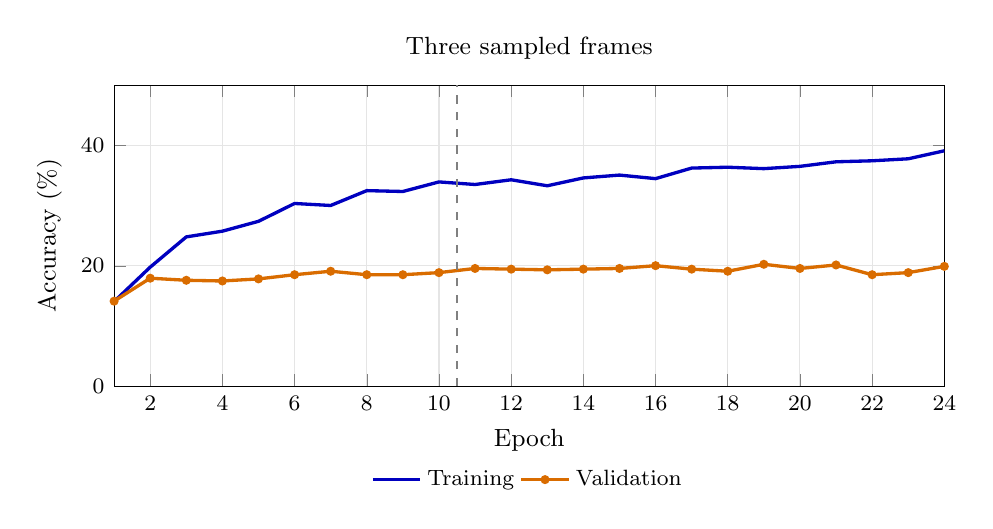
\begin{tikzpicture}
\begin{axis}[width=\textwidth,height=5.4cm,xmin=1,xmax=24,ymin=0,ymax=50,
 xlabel={Epoch},ylabel={Accuracy (\%)},title={Three sampled frames},
 grid=major,grid style={gray!20},tick label style={font=\footnotesize},
 label style={font=\small},title style={font=\small},
 legend style={font=\footnotesize,at={(0.5,-0.24)},anchor=north,legend columns=2,draw=none}]
\addplot[blue!75!black,very thick] coordinates { (1,14.055) (2,19.777) (3,24.810) (4,25.760) (5,27.398) (6,30.366) (7,30.033) (8,32.502) (9,32.360) (10,33.951) (11,33.523) (12,34.307) (13,33.310) (14,34.615) (15,35.090) (16,34.497) (17,36.254) (18,36.396) (19,36.159) (20,36.538) (21,37.298) (22,37.464) (23,37.797) (24,39.126) };
\addlegendentry{Training}
\addplot[orange!85!black,very thick,mark=*,mark size=1pt] coordinates { (1,14.120) (2,17.940) (3,17.593) (4,17.477) (5,17.824) (6,18.519) (7,19.097) (8,18.519) (9,18.519) (10,18.866) (11,19.560) (12,19.444) (13,19.329) (14,19.444) (15,19.560) (16,20.023) (17,19.444) (18,19.097) (19,20.255) (20,19.560) (21,20.139) (22,18.519) (23,18.866) (24,19.907) };
\addlegendentry{Validation}
\addplot[gray,dashed,forget plot] coordinates {(10.5,0)(10.5,50)};
\end{axis}
\end{tikzpicture}
\end{minipage}
\caption{Training and validation accuracy during the two ResNet50 runs. The dashed line marks the start of Phase 2 fine-tuning after epoch 10.}
\label{fig:resnet-curves}
\end{figure}

The skeleton ablations helped select the final settings. Table~\ref{tab:ablation} shows the validation accuracy averaged across five seeds. Ordered Model B performed better than its shuffled counterpart. Mirroring improved Model B validation accuracy. Adding video duration made almost no difference, so duration was omitted from the final setup.

\vspace{0.6em}
\begin{table}[H]
\centering
\small
\setlength{\tabcolsep}{10pt}
\renewcommand{\arraystretch}{1.20}
\arrayrulecolor{tableborder}
\caption{Skeleton validation comparisons, mean accuracy across five seeds.}
\label{tab:ablation}
\begin{tabular}{lc}
\toprule
\rowcolor{tablehead}
\textcolor{white}{\textbf{Configuration}} & \textcolor{white}{\textbf{Validation accuracy}} \\
\midrule
\rowcolor{tablerowlight}
Model A, single pose, mirroring on & 41.1\% \\
Model A, single pose, mirroring off & 40.6\% \\
\rowcolor{tablerowlight}
Model B, ordered, duration on, mirroring on & 66.5\% \\
\rowcolor{tablehighlight}
\textbf{Model B, ordered, duration off, mirroring on (Selected)} & \textbf{66.7\%} \\
\rowcolor{tablerowlight}
Model B, ordered, duration on, mirroring off & 60.6\% \\
Model B, shuffled, duration on, mirroring on & 55.9\% \\
\bottomrule
\end{tabular}
\end{table}

\clearpage
\subsection{Final test results}
The final evaluation used 288 videos from eight test players who were held out from both training and validation sets. For the photo pipeline, the midpoint-frame ResNet50 reached 30.56\% test accuracy. Scoring the three frames separately yielded 22.69\% accuracy across 864 individual test images. Averaging the three frame predictions per video reached 33.33\% accuracy across the 288 test videos.

For the skeleton pipeline, each result is reported as the mean and standard deviation across five independent training runs using seeds 42--46. The single-pose Model~A reached 43.6\% $\pm$ 1.1\%. The shuffled-sequence control reached 56.9\% $\pm$ 1.8\%, and the ordered Model~B reached 68.0\% $\pm$ 1.4\%. By comparison, random guessing across the 12 balanced classes corresponds to an expected baseline of 8.33\%.

\vspace{0.8em}
\begin{table}[H]
\centering
\small
\setlength{\tabcolsep}{8pt}
\renewcommand{\arraystretch}{1.22}
\arrayrulecolor{tableborder}
\caption{Test accuracy on the held-out player split. Skeleton results are mean $\pm$ standard deviation across five seeds.}
\label{tab:test}
\begin{tabular}{lcc}
\toprule
\rowcolor{tablehead}
\textcolor{white}{\textbf{Method}} & \textcolor{white}{\textbf{Evaluation unit}} & \textcolor{white}{\textbf{Test accuracy}} \\
\midrule
\rowcolor{tablerowlight}
ResNet50, one midpoint frame & 288 videos & 30.56\% \\
ResNet50, three frames scored separately & 864 images & 22.69\% \\
\rowcolor{tablerowlight}
ResNet50, three-frame prediction average & 288 videos & 33.33\% \\
Skeleton Model A, one midpoint pose & 288 videos & 43.6\% $\pm$ 1.1\% \\
\rowcolor{tablerowlight}
Skeleton shuffled-sequence control & 288 videos & 56.9\% $\pm$ 1.8\% \\
\rowcolor{tablehighlight}
\textbf{Skeleton Model B, ordered sequence} & \textbf{288 videos} & \textbf{68.0\% $\pm$ 1.4\%} \\
\bottomrule
\end{tabular}
\end{table}

\vspace{0.6em}
\begin{figure}[H]
\centering
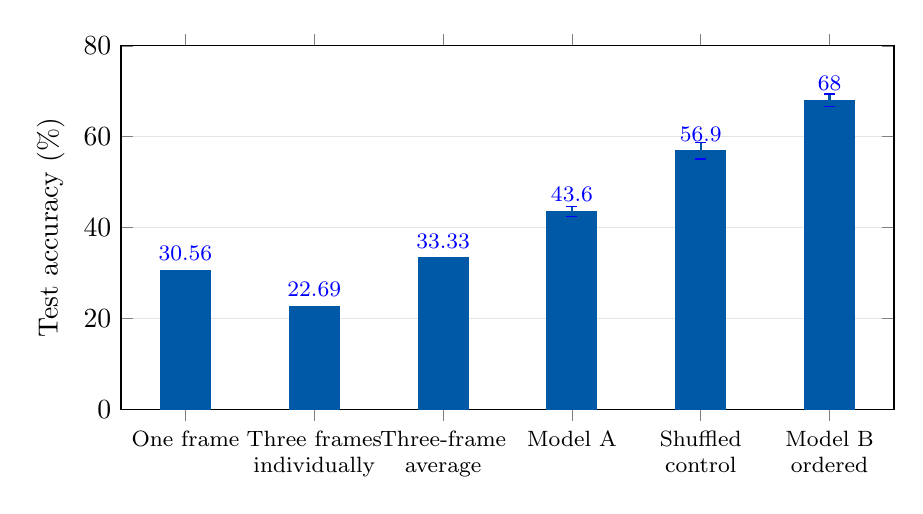
\begin{tikzpicture}
\begin{axis}[
 ybar,width=0.94\textwidth,height=6.2cm,bar width=18pt,
 ylabel={Test accuracy (\%)},ymin=0,ymax=80,
 symbolic x coords={f1,f3i,f3a,a,shuf,b},xtick=data,
 xticklabels={One frame,{Three frames\\individually},{Three-frame\\average},Model A,{Shuffled\\control},{Model B\\ordered}},
 xticklabel style={font=\footnotesize,align=center},
 ymajorgrids=true,grid style={gray!20},
 nodes near coords,nodes near coords style={font=\footnotesize,anchor=south}]
\addplot+[fill=teal!70!blue,draw=teal!70!blue,error bars/.cd,y dir=both,y explicit,error bar style={line width=0.8pt}] coordinates {
 (f1,30.56)
 (f3i,22.69)
 (f3a,33.33)
 (a,43.6) +- (0,1.1)
 (shuf,56.9) +- (0,1.8)
 (b,68.0) +- (0,1.4)
};
\end{axis}
\end{tikzpicture}
\caption{Test accuracy for the photo and skeleton approaches. The first three bars show ResNet50 results; the last three show skeleton results. Error bars show the standard deviation across five seeds for skeleton models. The three-frame individual score is measured over 864 images; the other results are measured over 288 videos.}
\label{fig:test-bars}
\end{figure}

The three-frame averaging result of 33.33\% does not represent temporal learning: it merely aggregates three independent static frame predictions. In contrast, the skeleton models provide direct empirical evidence regarding the necessity of chronological motion dynamics. Ordered Model~B achieved 68.0\% $\pm$ 1.4\% test accuracy, substantially outperforming the single-pose Model~A baseline (43.6\% $\pm$ 1.1\%) by +24.4 percentage points. 

Crucially, Model~B also outperformed the shuffled-sequence control (56.9\% $\pm$ 1.8\%) by +11.1 percentage points. Because the shuffled control receives identical spatial coordinate landmarks and posture statistics with only temporal order randomized, this +11.1\% margin specifically isolates the contribution of chronological trajectory ordering. Furthermore, when the trained ordered Model~B was evaluated with test sequence frames randomly shuffled at inference time, its accuracy plummeted to 41.4\% $\pm$ 1.6\%, near the single-frame baseline. These findings confirm that Model~B relies heavily on chronological kinematic transitions rather than merely acting as an ensemble over static postures.

\subsection{Class-wise errors}
A granular examination of classification patterns reveals distinct failure modes across visual and kinematic representations. The confusion matrices for all evaluated models are presented across the following two pages: Figure~\ref{fig:cm-1frame} and Figure~\ref{fig:cm-3frame} display the ResNet50 one-frame and three-frame confusion matrices (page~\pageref{fig:cm-1frame}), while Figure~\ref{fig:cm-skel-A} and Figure~\ref{fig:cm-skel-B} illustrate the single-pose Model~A and sequence-based Model~B skeleton confusion matrices (page~\pageref{fig:cm-skel-A}).

Across the photo pipeline (Figures~\ref{fig:cm-1frame} and~\ref{fig:cm-3frame}), widespread misclassifications occur between forehands and backhands, as static visual snapshots cannot differentiate stroke direction without temporal context. In contrast, the skeleton Model~B (Figure~\ref{fig:cm-skel-B}) achieves its strongest recognition rates on dynamic groundstrokes (\texttt{backhand}, \texttt{backhand2hands}, \texttt{forehand\_flat}, \texttt{forehand\_openstands}), where full-body pelvic and shoulder rotations provide unmistakable kinematic signatures. 

However, all models exhibit persistent confusion within the service cluster (\texttt{flat\_service}, \texttt{kick\_service}, \texttt{slice\_service}). These actions share virtually identical preparatory stances, knee flexion, and overhead ball-toss trajectories. Because THETIS videos do not capture the tennis ball and the pose estimator does not track racquet face angle or wrist pronation during ball impact, the visual and kinematic cues available to discriminate service spin variations remain severely constrained.

\clearpage
\begin{figure}[H]
\centering
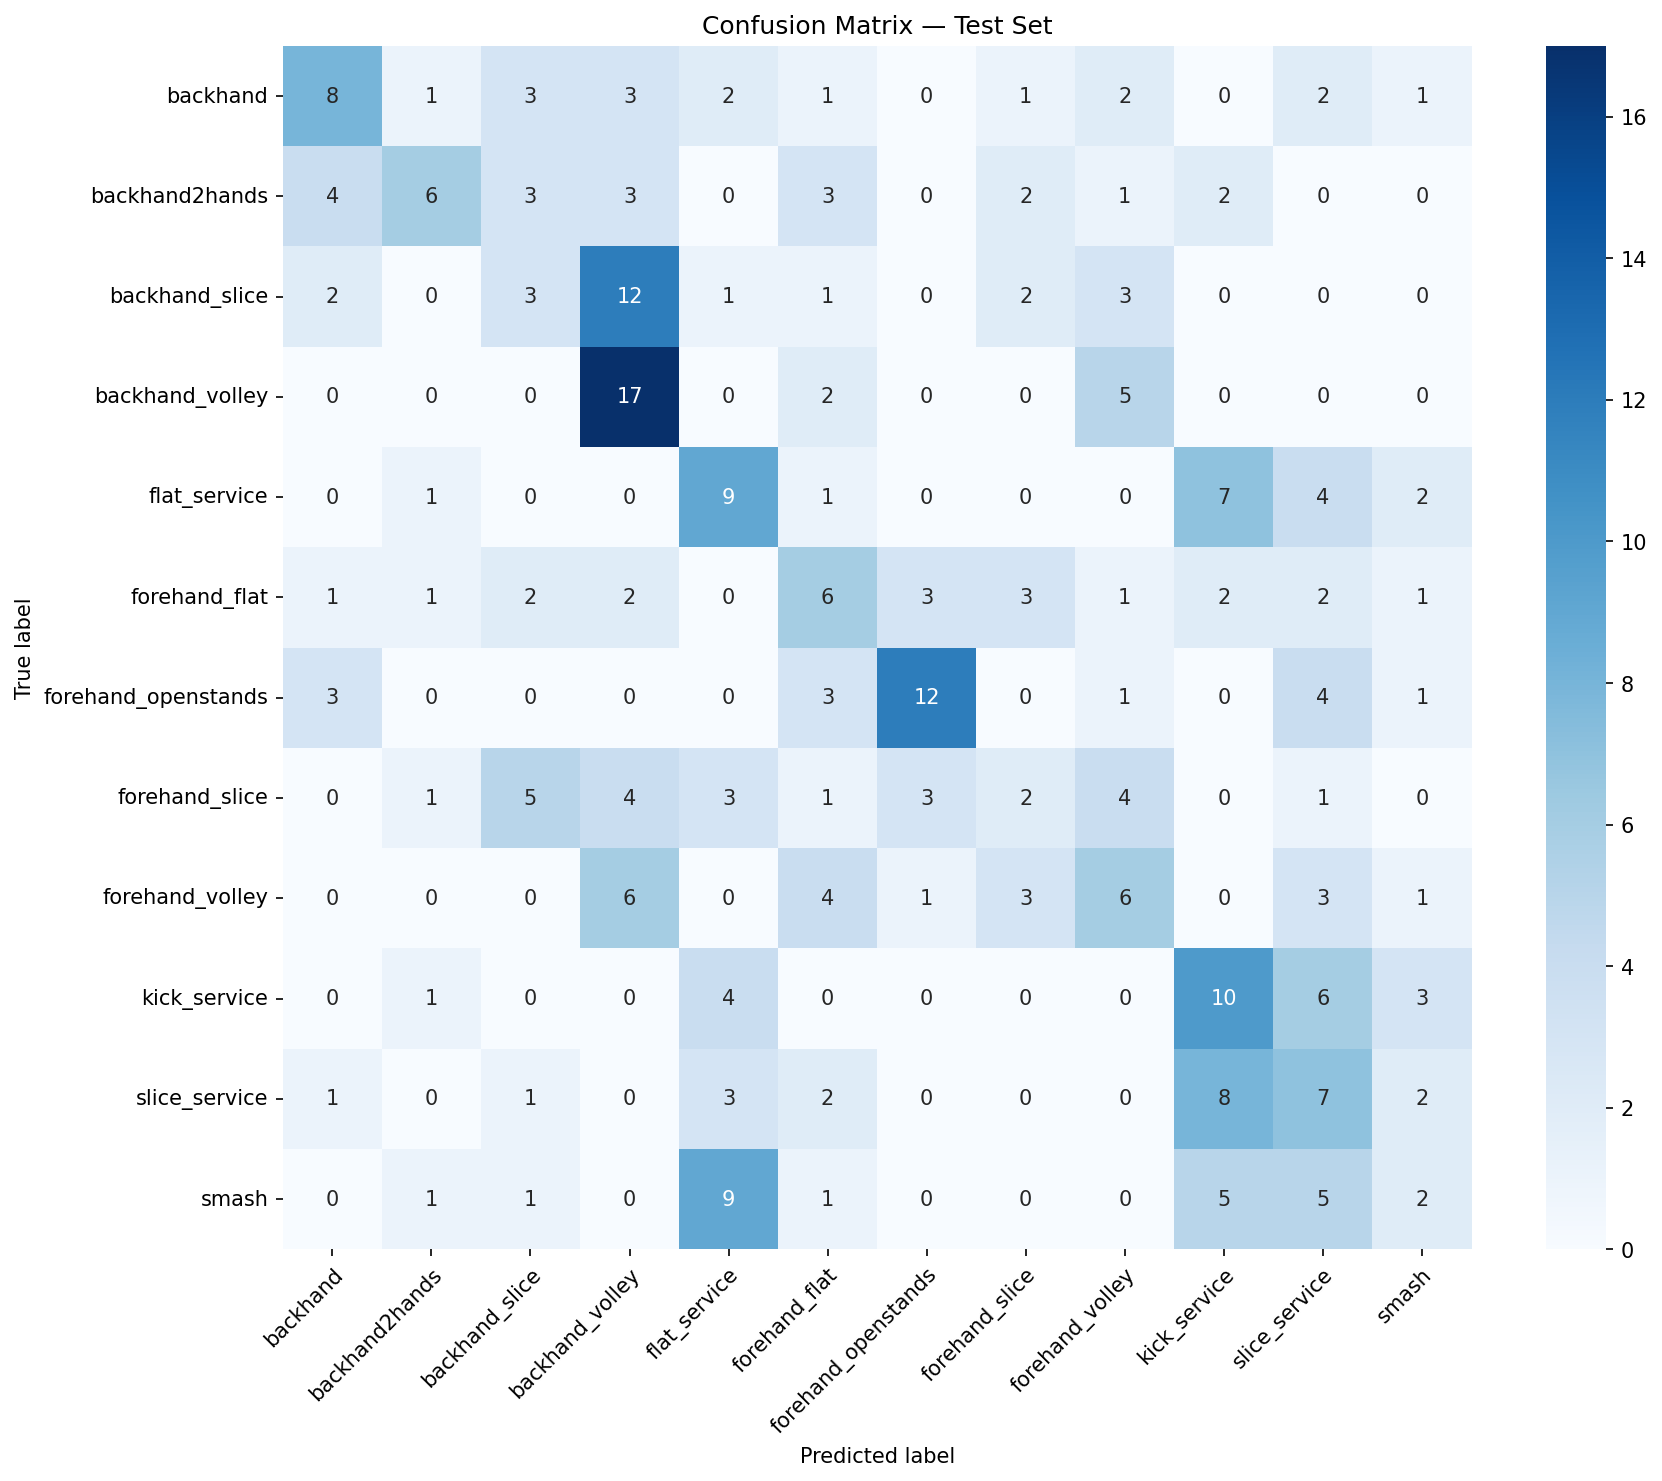
\includegraphics[height=10.2cm]{confusion_matrix_1frame.png}
\caption{ResNet50 test confusion matrix using one midpoint frame.}
\label{fig:cm-1frame}
\end{figure}
\begin{figure}[H]
\centering
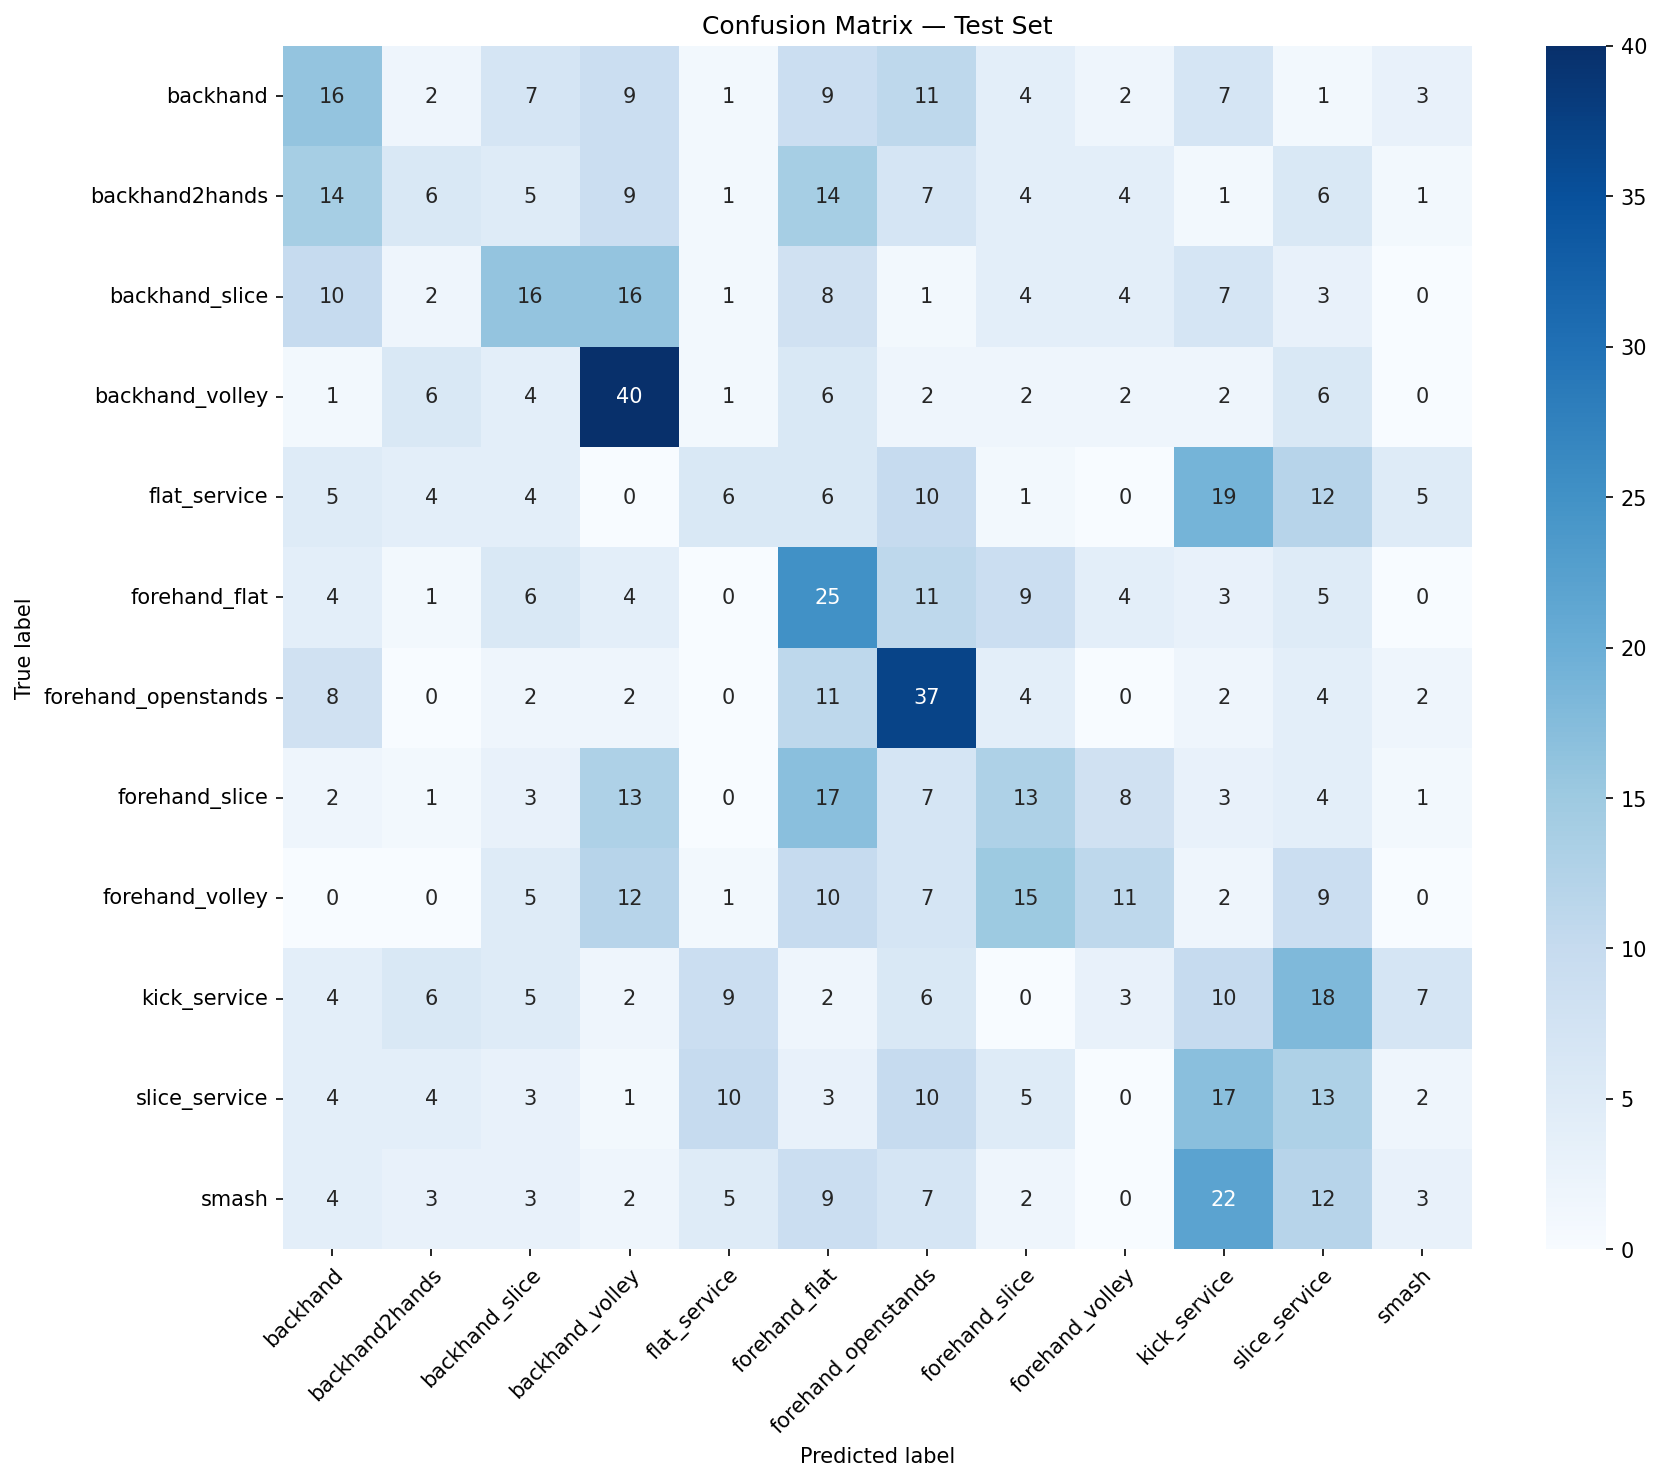
\includegraphics[height=10.2cm]{confusion_matrix_3frame.png}
\caption{ResNet50 test confusion matrix for three frames scored individually.}
\label{fig:cm-3frame}
\end{figure}

\clearpage
\begin{figure}[H]
\centering
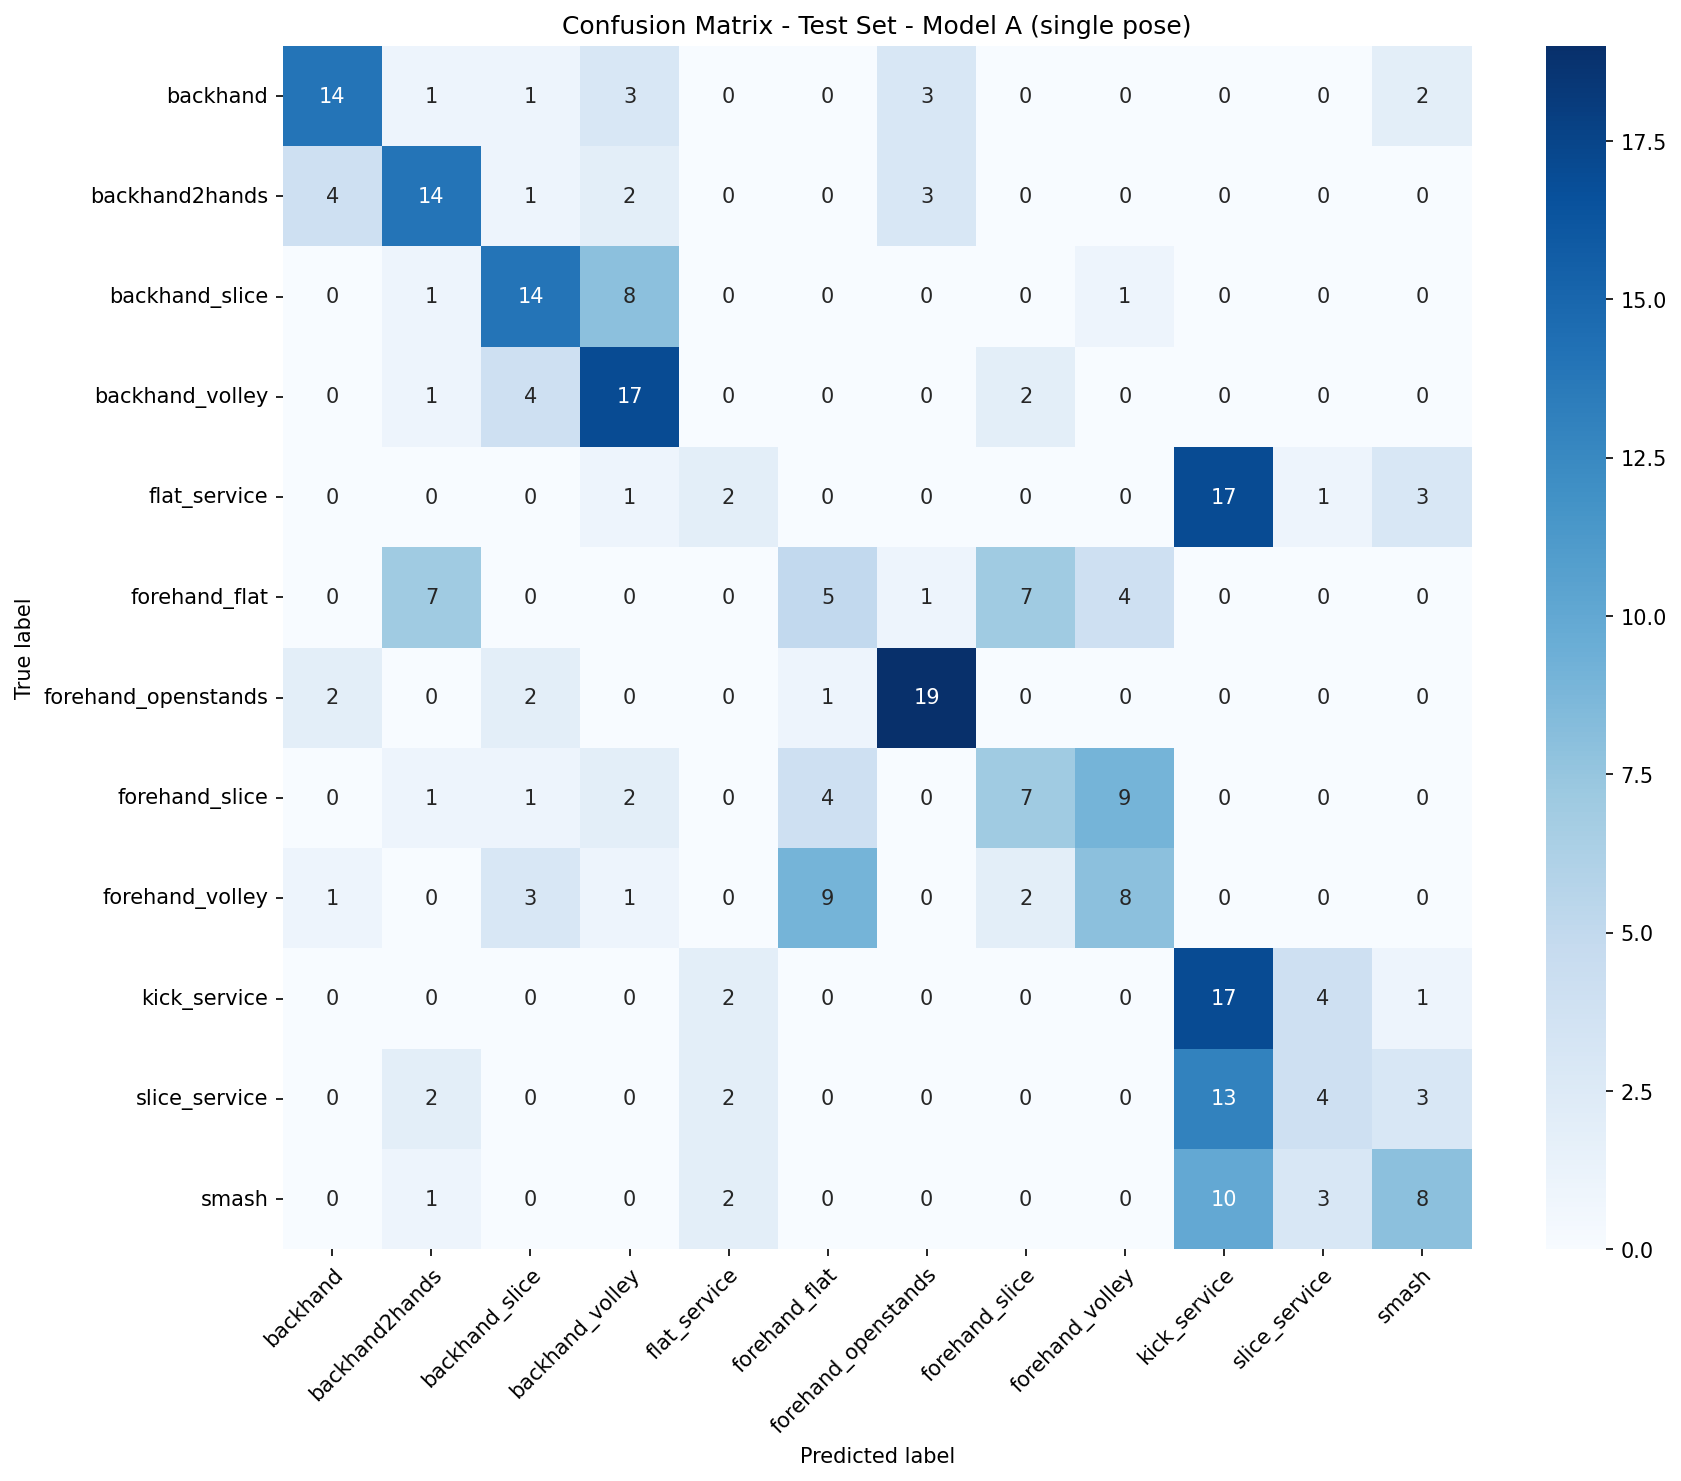
\includegraphics[height=10.2cm]{test_confusion_A.png}
\caption{Skeleton Model A test confusion matrix for seed 42 (44.79\% accuracy).}
\label{fig:cm-skel-A}
\end{figure}
\begin{figure}[H]
\centering
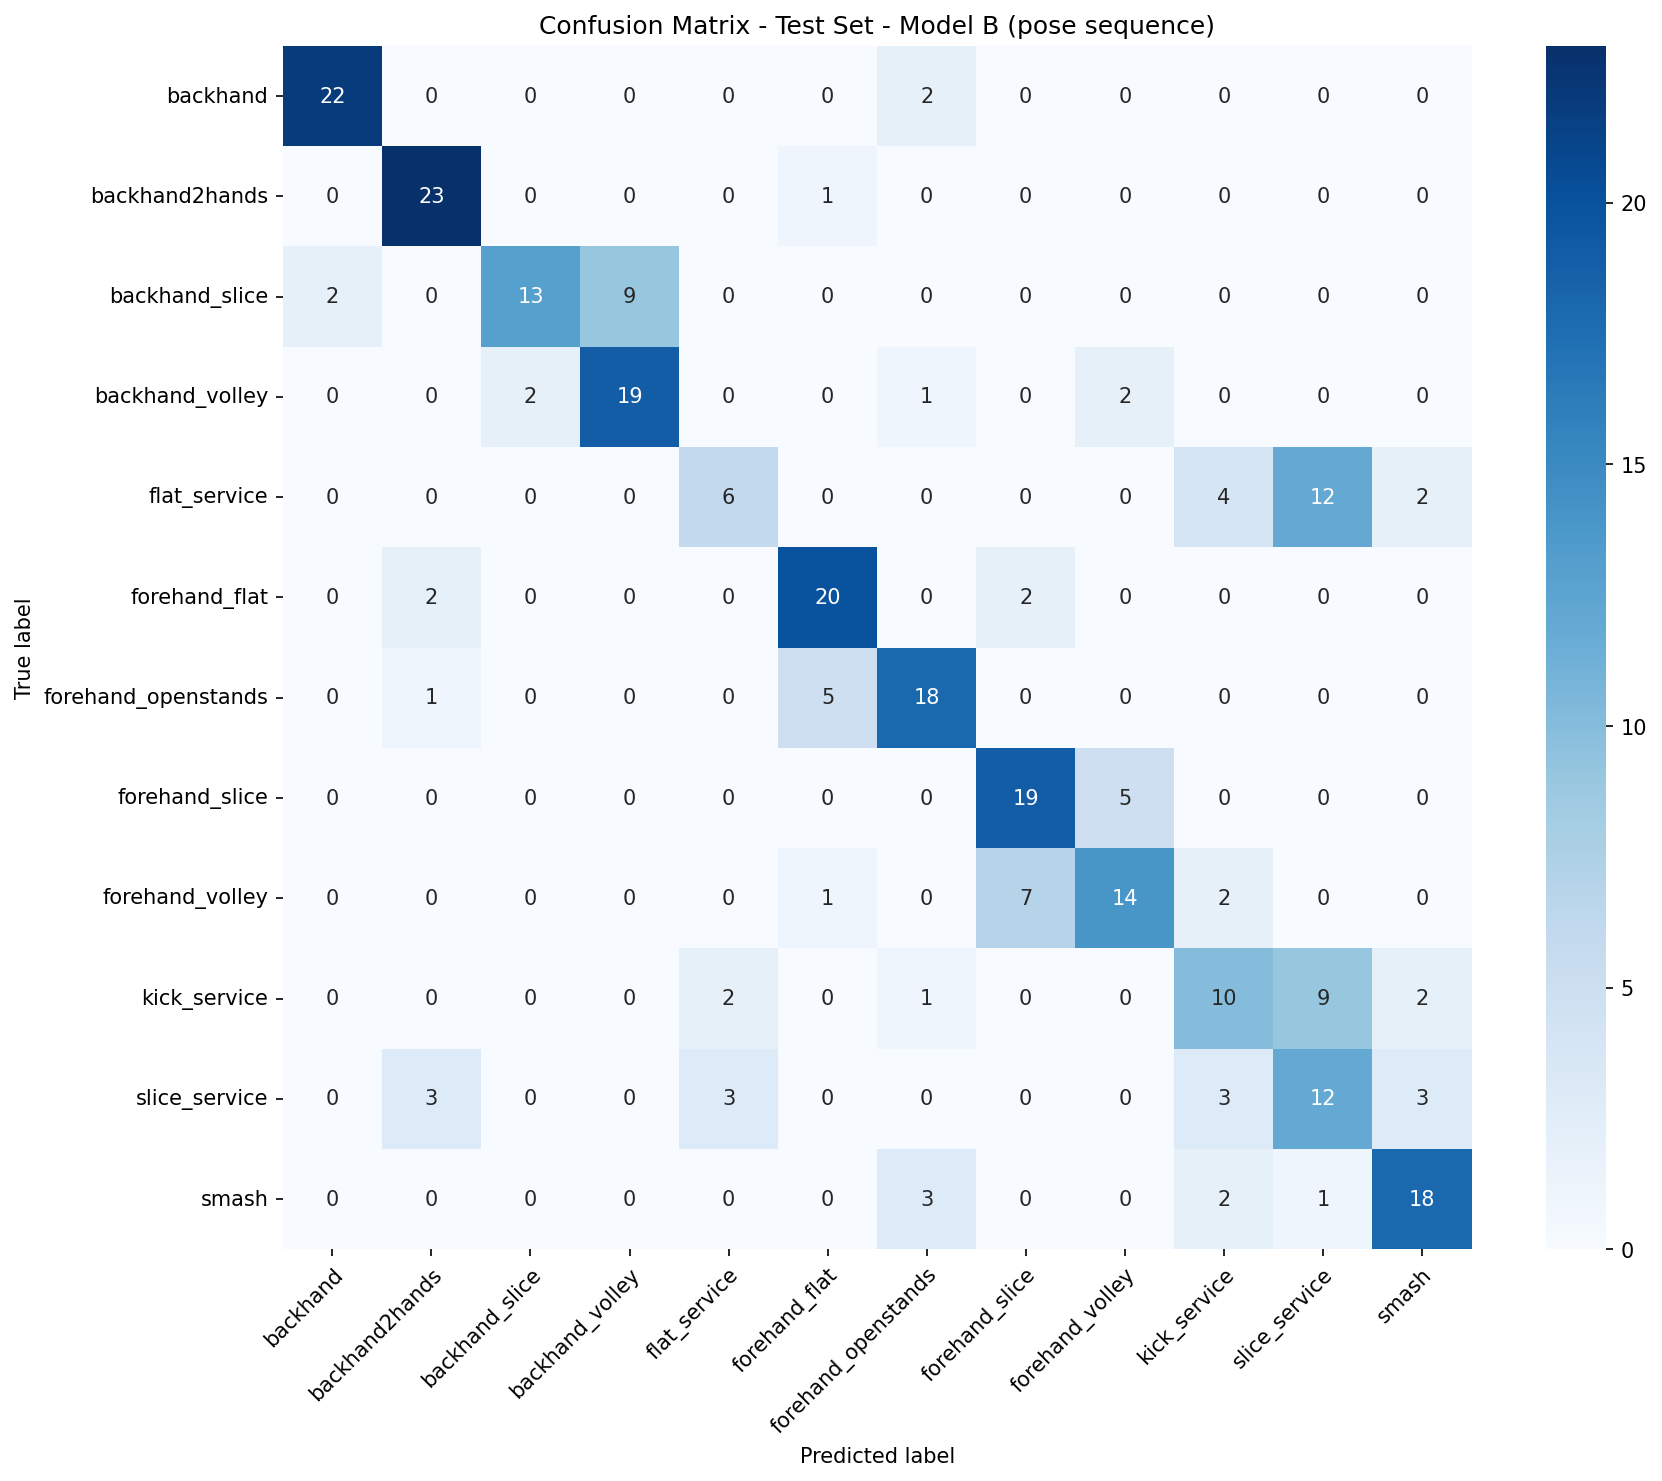
\includegraphics[height=10.2cm]{test_confusion_B.png}
\caption{Ordered Skeleton Model B test confusion matrix for seed 42 (67.36\% accuracy).}
\label{fig:cm-skel-B}
\end{figure}

\clearpage
\subsection{Limitations}
The empirical conclusions of this project must be interpreted in light of several methodological and domain-specific limitations. First, regarding dataset scope, THETIS consists of staged indoor recordings captured in an invariant gymnasium environment with a static Kinect camera. Although the dataset includes 55 distinct subjects, players performed strokes in isolation without active opponent rallies, ball bounces, or court movement. Consequently, the models were evaluated on isolated athletic choreography rather than in-situ tennis match dynamics.

Second, the absence of ball trajectory and equipment telemetry represents a major bottleneck for fine-grained discrimination. Tennis strokes are fundamentally characterized by ball velocity, trajectory curvature, impact timing, and racquet face orientation. Because low video frame rates (17--18 fps) and motion blur render the tennis ball invisible and prevent racquet angle segmentation, neither the image-based nor the skeleton-based pipeline received equipment-level cues. This directly accounts for the persistent confusion among flat, kick, and slice services, which share near-identical full-body preparatory stances but diverge solely in subtle wrist pronation and racquet path during contact.

Third, pose estimation quality introduces downstream sensor noise. While Ultralytics YOLO11m-pose substantially improved joint fidelity over the native Kinect skeletal streams, 2D landmark localization remains susceptible to self-occlusion during complex two-handed backhands or extreme rotational follow-throughs. Although temporal linear interpolation repaired sporadic tracking dropouts, unmodeled joint jitters can distort velocity profiles in fast arm swings.

Fourth, the experimental comparison between photo and skeleton pipelines is methodologically asymmetric. ResNet50 operated on static 2D image snapshots (one or three frames) and underwent conservative two-phase fine-tuning with frozen batch-normalization statistics, reaching modest training accuracy. In contrast, Model~B operated on a temporally normalized 64-step sequence across all 17 anatomical landmarks and was trained end-to-end. Hence, the performance gap reflects not only modality differences (raw pixels vs.\ joint coordinates) but also temporal sequence availability. Finally, all evaluations were conducted on a single fixed 39/8/8 subject split; while seeds 42--46 varied stochastic training initialization, variance across different player cohort groupings was not evaluated.

\clearpage
\section{Conclusion}
This mini-project investigated fine-grained sports human action recognition by directly comparing appearance-based deep transfer learning with kinematic sequence modeling on the 12-class THETIS tennis benchmark. The original investigation implemented an ImageNet-pretrained ResNet50 classifier evaluated on single midpoint keyframes and three-frame multi-view ensembles. To overcome the vulnerability of static visual representations to background and clothing biases, a dedicated skeleton-based extension was developed. This secondary pipeline recovered 17 anatomical landmarks using YOLO11m-pose, applied spatial hip-centering and torso-scale normalization, resampled clips to 64 uniform time steps, and classified full movement trajectories with a 1D Temporal Convolutional Network (Model~B).

Under a strict 39/8/8 subject-wise evaluation protocol that completely prevents player identity leakage, the static ResNet50 achieved 30.56\% test accuracy on single midpoint frames and 33.33\% via three-frame prediction averaging across 288 held-out videos. In sharp contrast, the kinematic pipeline achieved 43.6\% $\pm$ 1.1\% on single midpoint poses (Model~A) and reached 68.0\% $\pm$ 1.4\% using the full ordered 64-step sequence (Model~B). Crucially, a controlled temporal shuffle experiment (56.9\% $\pm$ 1.8\%) and inference-time sequence corruption (dropping to 41.4\% $\pm$ 1.6\%) empirically verified that chronological trajectory dynamics contribute a decisive +11.1 percentage point performance dividend over static posture ensembles.

These results demonstrate that compact kinematic representations successfully filter out environmental nuisance factors while capturing fine-grained athletic biomechanics at a fraction of the computational footprint required by volumetric 3D-CNNs. Nevertheless, recognizing subtle service variations remains challenging without ball trajectory or racquet orientation data.

Future investigations should focus on four prospective directions: first, extending subject-wise cross-validation across multiple randomized cohort partitions to assess demographic generalization; second, incorporating multimodal sensor fusion combining body pose with high-speed ball tracking and racquet-mounted inertial measurement units (IMUs); third, exploring graph convolutional architectures (ST-GCN) and spatio-temporal attention transformers operating on 3D lifted joints; and fourth, validating the framework on real-world broadcasting footage featuring unconstrained camera motion and live matchplay.

\clearpage
\begin{thebibliography}{9}
\bibitem{gourgari2013thetis} S. Gourgari, G. Goudelis, K. Karpouzis, and S. Kollias, ``\href{https://openaccess.thecvf.com/content_cvpr_workshops_2013/W08/papers/Gourgari_THETIS_Three_Dimensional_2013_CVPR_paper.pdf}{THETIS: Three Dimensional Tennis Shots a Human Action Dataset},'' in \emph{Proceedings of the IEEE Conference on Computer Vision and Pattern Recognition Workshops}, pp. 676--681, 2013. doi: 10.1109/CVPRW.2013.102.
\bibitem{he2016deep} K. He, X. Zhang, S. Ren, and J. Sun, ``\href{https://openaccess.thecvf.com/content_cvpr_2016/html/He_Deep_Residual_Learning_CVPR_2016_paper.html}{Deep Residual Learning for Image Recognition},'' in \emph{Proceedings of the IEEE Conference on Computer Vision and Pattern Recognition}, pp. 770--778, 2016. doi: 10.1109/CVPR.2016.90.
\bibitem{russakovsky2015imagenet} O. Russakovsky et al., ``\href{https://doi.org/10.1007/s11263-015-0816-y}{ImageNet Large Scale Visual Recognition Challenge},'' \emph{International Journal of Computer Vision}, vol. 115, no. 3, pp. 211--252, 2015.
\bibitem{hovad2024classification} E. Hovad, T. Hougaard-Jensen, and L. K. H. Clemmensen, ``\href{https://arxiv.org/abs/2402.02545}{Classification of Tennis Actions Using Deep Learning},'' arXiv:2402.02545, 2024.
\bibitem{feichtenhofer2019slowfast} C. Feichtenhofer, H. Fan, J. Malik, and K. He, ``\href{https://openaccess.thecvf.com/content_ICCV_2019/html/Feichtenhofer_SlowFast_Networks_for_Video_Recognition_ICCV_2019_paper.html}{SlowFast Networks for Video Recognition},'' in \emph{Proceedings of the IEEE/CVF International Conference on Computer Vision}, pp. 6202--6211, 2019.
\bibitem{jocher2024yolo11} G. Jocher and J. Qiu, ``Ultralytics YOLO11,'' software, 2024. Available: \url{https://github.com/ultralytics/ultralytics}.
\bibitem{lin2014microsoft} T.-Y. Lin et al., ``\href{https://doi.org/10.1007/978-3-319-10602-1_48}{Microsoft COCO: Common Objects in Context},'' in \emph{Computer Vision -- ECCV 2014}, pp. 740--755, 2014. doi: 10.1007/978-3-319-10602-1\_48.
\bibitem{kingma2015adam} D. P. Kingma and J. Ba, ``\href{https://arxiv.org/abs/1412.6980}{Adam: A Method for Stochastic Optimization},'' in \emph{International Conference on Learning Representations}, 2015. arXiv:1412.6980.
\end{thebibliography}

\end{document}